\section{Problem Examples}

\begin{frame}
  \frametitle{Problem Example: 191 -- Intersection}
    \begin{block}{Summary}
      \begin{itemize}
      \item {\bf Input}: A rectangle and a line segment:
        \begin{itemize}
          \item Rectangle: $x_s y_s x_e y_e$
          \item Line: $x_0, y_0, x_1, y_1$
        \end{itemize}

      \item {\bf Output}\\
        T - if the line segment intersects the rectangle\\
        F - if the line segment does not intersect the rectangle\\
      \end{itemize}
    \end{block}
    \begin{columns}
      \column{.3\textwidth}
      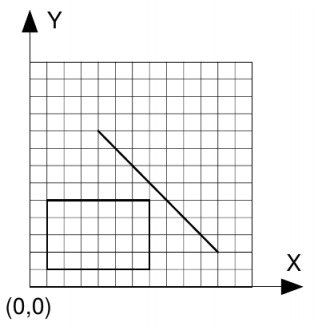
\includegraphics[width=1\textwidth]{img/intersection_uva}
      \ppagenote{Problem image from \url{https://onlinejudge.org}}
      \column{.7\textwidth}
      How do you solve it?
    \end{columns}

\end{frame}

\begin{frame}
  \frametitle{Problem Example: 191 -- Intersection}

  \begin{columns}
    \column{.45\textwidth}
    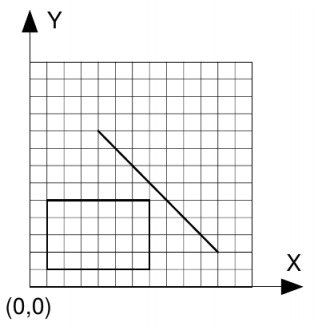
\includegraphics[width=\textwidth]{img/intersection_uva}
    \column{.55\textwidth}

    \begin{itemize}
      \item Test if $p_1$ or $p_2$ are inside the rectangle;
      \item For each segment $\overline{AB}$, test if $\overline{p_1,p_2}$ intersects $\overline{AB}$.\bigskip

      \item (optional) make a videogame;
    \end{itemize}
  \end{columns}
\end{frame}

\begin{frame}
  \frametitle{Problem Example: 833 -- Waterfalls}
    \begin{block}{Summary}
      \begin{itemize}
      \item {\bf Input}
      \begin{itemize}
        \item List of line segments that block water;
        \item List of water sources;
      \end{itemize}

      \item {\bf Output}
      \begin{itemize}
        \item For every waterfall w, the end position $X_w$ where $Y_w=0$
      \end{itemize}
      \end{itemize}
    \end{block}

    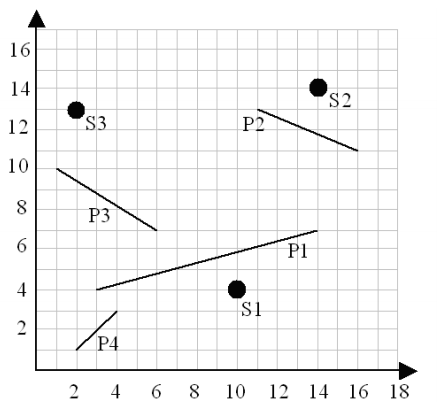
\includegraphics[width=0.35\textwidth]{img/waterfall}
    \ppagenote{Problem image from \url{https://onlinejudge.org}}
\end{frame}

\begin{frame}
  \frametitle{Problem Example: UVA 833 -- Waterfalls}
  \begin{columns}
    \column{0.4\textwidth}
      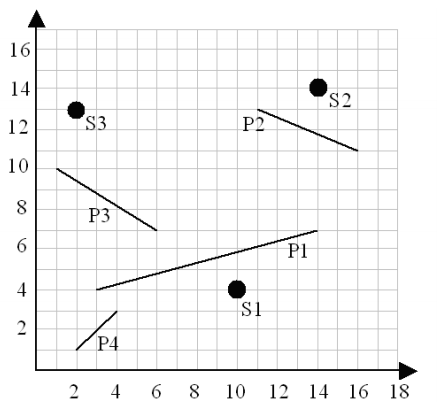
\includegraphics[width=1\textwidth]{img/waterfall}
    \column{0.6\textwidth}
    {\bf Full Search:}
    \begin{itemize}
      \item For each water source $S_i$:
      \begin{itemize}
        \item Calculate which segment intersects $\overline{S_i0}$ first.
        \item Adjust the position $X_i$ and repeat until $Y_i = 0$.
      \end{itemize}\bigskip

      \item This is a bit slow if there are many sources and segments.
      \item Can you pre-calculate something?
      \item Remember that all inputs are integers!
    \end{itemize}
  \end{columns}
\end{frame}

\section{Basic Functions}
\begin{frame}
  \centering
  {\bf Basic Functions -- Points and Lines}
\end{frame}

\subsection{Points}
\begin{frame}[fragile]{Point Representation}
    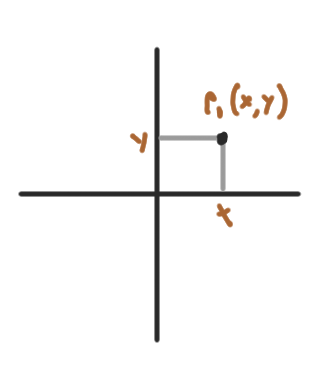
\includegraphics[width=.2\textwidth]{../img/geom2}
    \begin{exampleblock}{}
\begin{verbatim}
struct point_i { int x, y;  // integer coordinates
  point_i() { x = y = 0; }
  point_i(int _x, int _y) : x(_x), y(_y) {}};

struct point { double x, y; // double coordinates
  point() { x = y = 0.0;}
  point(double _x, double _y) : x(_x), y(_y) {}};
\end{verbatim}
    \end{exampleblock}
\end{frame}

\begin{frame}[fragile]{Overloading Point Operators}

    \begin{exampleblock}{Point Operators}
\begin{verbatim}
struct point { double x, y;
   point() { x = y = 0.0;
   point(double _x, double _y) : x(_x), y(_y) {}

   // Overloading "<" to sort by coordinate
   bool operator < (point other) const {
      if (fabs(x - other.x) > EPS)
         return x < other.x;
      return y < other.y; }
   // Overloading "==" for equality testing
   bool operator == (point other) const {
      return (fabs(x - other.x) < EPS &&
             (fabs(y - other.y) < EPS)); }
   }
\end{verbatim}
    \end{exampleblock}
\end{frame}

\begin{frame}[fragile]{Point Distance}
    \begin{exampleblock}{}
\begin{verbatim}
            // Euclidean Distance: "normal" distance
#define hypot(dx,dy) sqrt(dx*dx + dy*dy)
double dist(point p1, point p2) {
  return hypot(p1.x - p2.x, p1.y - p2.y); }
            // Taxicab Distance: Distance on a grid
double taxicab(point p1, point p2) {
  return fabs(p1.x - p2.x) + fabs(p1.y - p2.y); }
\end{verbatim}
    \end{exampleblock}

    \begin{center}
      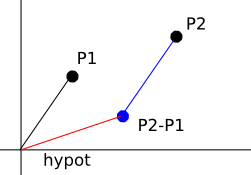
\includegraphics[width=0.4\textwidth]{../img/geom1}
    \end{center}
\end{frame}

\begin{frame}[fragile]{Point Rotation}

  {\smaller

    \begin{exampleblock}{}
\begin{verbatim}
#define PI           3.14159265358979323846 // Pi constant
double PI = 2 * acos(0.0)                   // Better Pi
#define DEG_to_RAD(X) (X*PI)/180.0

// angle t is in degrees (0--360)
point rotate(point p, double t) {
   double rad = DEG_to_RAD(t);
   return point(p.x * cos(rad) - p.y * sin(rad),
                p.x * sin(rad) + p.y * cos(rad));}
\end{verbatim}
    \end{exampleblock}
    \begin{center}
      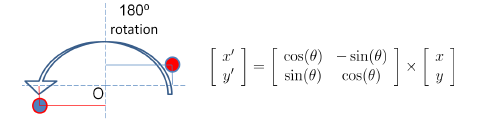
\includegraphics[width=0.8\textwidth]{../img/rotation_halim}
      \ppagenote{Rotation Image from "Competitive Programming 3", Steven Halim}
    \end{center}
}
    {\bf Quiz:} How do you rotate a point around $x_1, y_1$?
\end{frame}

\subsection{Lines}

\begin{frame}[fragile]
  \frametitle{Line Basics}
  How to represent a line:
  \begin{itemize}
  \item \structure{$ax + by + c = 0$}\hfill (a,b,c) -- useful for most cases
  \item \structure{$y = mx + c$}\hfill (m,c) -- useful for angle manipulation
  \item \structure{$x_0,y_0,x_1,y_1$}\hfill ($p_1, p_2$) -- harder to use, but common input
  \end{itemize}

{\smaller
  \begin{exampleblock}{How to convert from two points to a line}
\begin{verbatim}
struct line { double a,b,c; };

void pointsToLine(point p1, point p2, line &l) {
   if (fabs(p1.x - p2.x) < EPS {
      l.a = 1.0; l.b = 0.0; l.c = -p1.x; }
   else {
      l.a = -(double) (p1.y - p2.y)/(p1.x - p2.x);
      l.b = 1.0; l.c = -(double) (l.a*p1.x) - p1.y;}
}
\end{verbatim}
  \end{exampleblock}
  }
\end{frame}

\begin{frame}[fragile]
  \frametitle{Line Equality}
    \begin{columns}
      \column{0.6\textwidth}
      \begin{itemize}
      \item We define a line as $a,b,c|(ax+by=c)$

      \item Two lines are parallel if their coefficients $(a, b)$ are the same;\medskip

      \item Two lines are identical if all coefficients $(a,b,c)$ are the same;
      \end{itemize}
      \column{0.4\textwidth}
      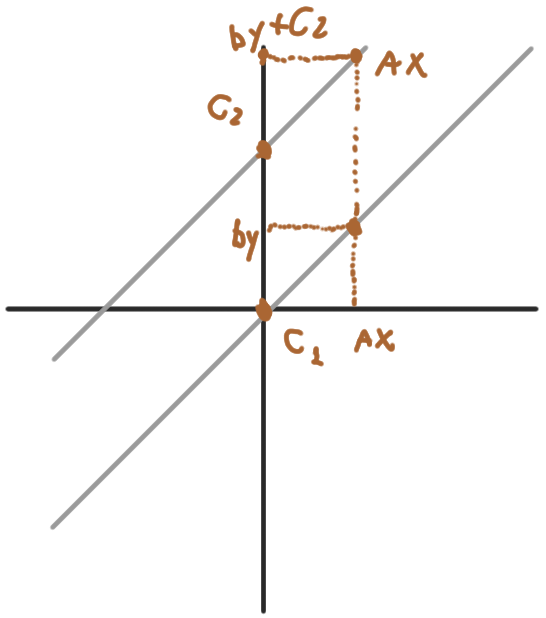
\includegraphics[width=.7\textwidth]{../img/geom3}
    \end{columns}
  \begin{exampleblock}{}
\begin{verbatim}
bool areParallel(line l1, line l2) {
   return (fabs(l1.a-l2.a) < EPS) &&
          (fabs(l1.b-l2.b) < EPS); }

bool areSame(line l1, line l2) {
   return areParallel(l1,l2) &&
          (fabs(l1.c - l2.c) < EPS); }
\end{verbatim}
  \end{exampleblock}
\end{frame}

\begin{frame}[fragile]
  \frametitle{Line Intersection}
    The intersection point $x_I, y_I$ can be found by solving:
    \begin{eqnarray*}
      a_1x_I+b_1y_I+c_1 = 0\\a_2x_I+b_2y_I+c_2 = 0
    \end{eqnarray*}
    Remember that when we create a line $i$, we set $b_i=0$ or $b_i=1$

    {\smaller
    \begin{exampleblock}{}
\begin{verbatim}
bool areIntersect(line l1, line l2, point &p) {
   if (areParallel(l1,l2)) return False;

   p.x = (l2.b * l1.c - l1.b * l2.c) /
         (l2.a * l1.b - l1.a * l2.b);

   // Test for vertical case:
   if (fabs(l1.b) > EPS)     p.y = -(l1.a * p.x + l1.c);
   else                      p.y = -(l2.a * p.x + l2.c);
   return True;
}
\end{verbatim}
    \end{exampleblock}

  }
\end{frame}

\subsection{Segments}
\begin{frame}[fragile]
  \frametitle{Segments and Vectors}
    \begin{columns}
      \column{0.8\textwidth}
      \begin{itemize}
        \item A {\bf line segment} is a line with two endpoints $(p_1, p_2)$ and finite length;
        \item A {\bf Vector} is a line segment with a direction;
        \begin{itemize}
          \item Usually represented as "direction" and "magnitude";
          \item Direction is a point with distance 1 from $(0,0)$
          \item Magnitude is a multiplier to the size of the vector;
          \item Represent movement, translation, speed, etc;
        \end{itemize}
      \end{itemize}
      \column{0.2\textwidth}
      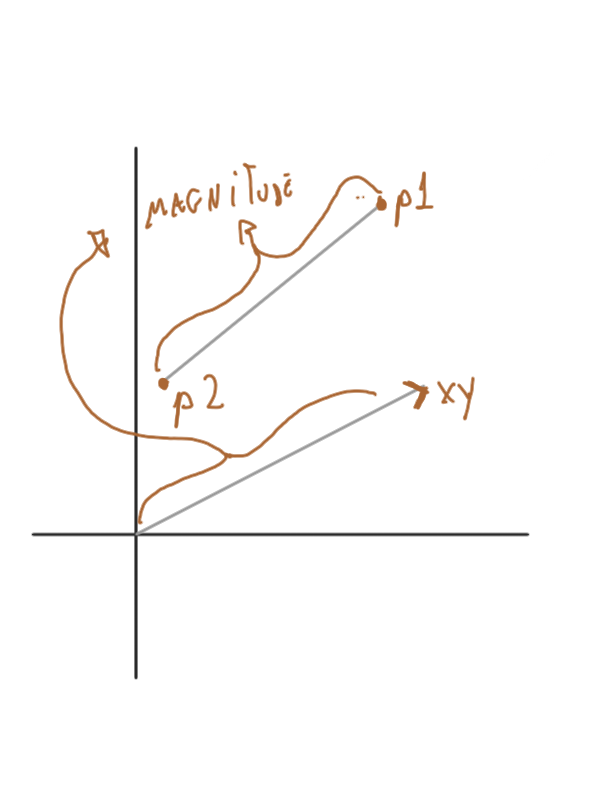
\includegraphics[width=.9\textwidth]{../img/geom4}
    \end{columns}

{\smaller
    \begin{exampleblock}{}
\begin{verbatim}
struct vec { double x, y;
    vec(double _x, double _y) : x(_x), y(_y) {} };

vec toVec(point a, point b) {
    return vec(b.x - a.x, b.y - a.y); }
vec scale(vec v, double s) {
    return vec(v.x * s, v.y * s); }
point translate(point p, vec v) {
    return point(p.x + v.x , p.y + v.y); }
\end{verbatim}
    \end{exampleblock}
  }
\end{frame}

\begin{frame}
  \frametitle{Distance between point and line, point and segment}
  \begin{block}{}
    For a point $p$ and a line $l$ (represented by $\overline{ab}$), the distance between both is given by the segment $pc$, where $c$ is the projection of $p$ in $l$.\bigskip

    {\smaller
    \begin{columns}[T]
      \column{.5\textwidth}
      Calculating $c$:
      \begin{itemize}
        \item calculate scalar proj. $u$ of $\vec{ap}$ in $l$.
        \item change magnitude of $\vec{ab}$ to $u$ to obtain $\vec{ac}$.
        \item calculate distance between $p$ and $c$.
      \end{itemize}
      \column{.5\textwidth}
      Distance between $p$ and $\overline{ab}$:
      \begin{itemize}
        \item calculate scalar proj. $u$ of $\vec{ap}$ in $l$.
        \item if $u < 0$ or $u > |\vec{ab}|$, then the distance is $\min(d(a,p),d(b,p))$.
        \item else, calculate $\vec{ac}$ and calculate distance $d(p,c)$.
      \end{itemize}
    \end{columns}}
  \end{block}

  \begin{center}
    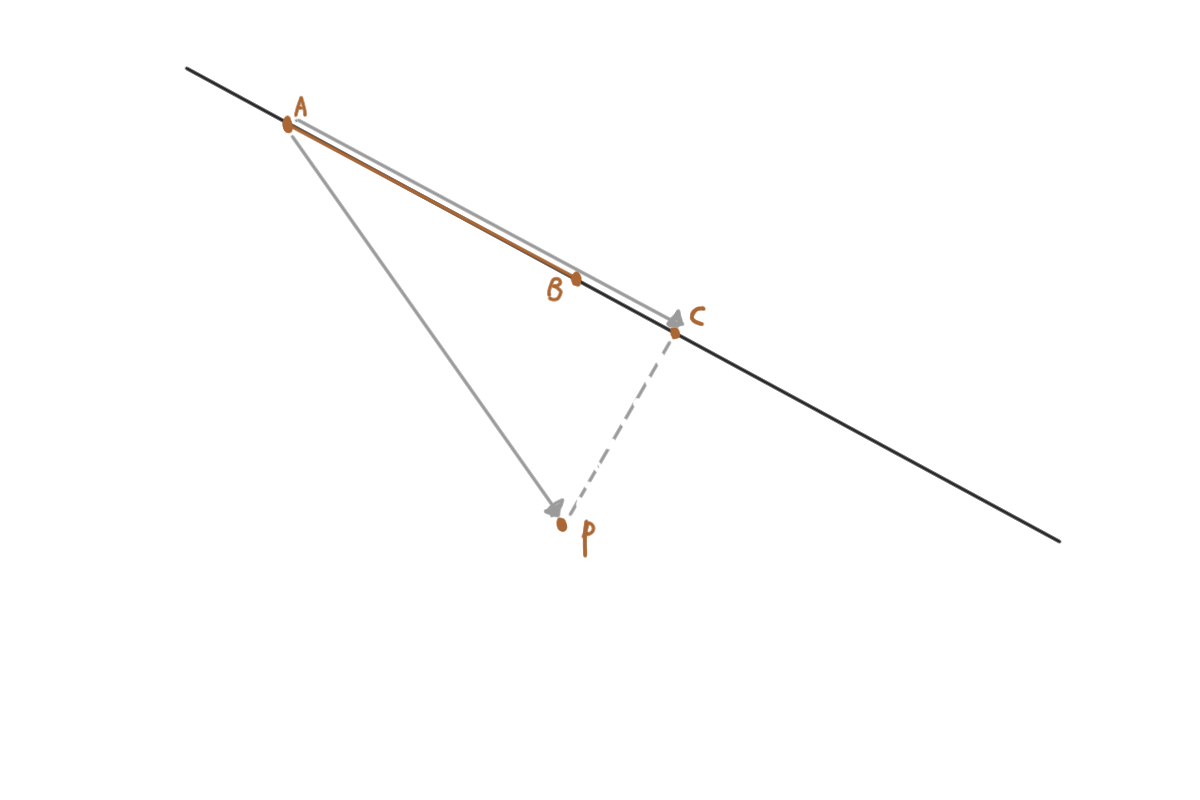
\includegraphics[width=0.5\textwidth]{../img/geom5}
  \end{center}
\end{frame}

\begin{frame}[fragile]
  \frametitle{CODE: Distance between point and line}

  {\smaller
  \begin{exampleblock}{}
\begin{verbatim}
double dot(vec a, vec b) {              // dot product
   return (a.x * b.x + a.y * b.y); }
double norm_sq(vec v) {                 // norm squared
   return v.x * v.x + v.y * v.y; }

// Given points a,b,p, calculate distance from p to line ab.
double distToLine(point p, point a, point b, point &c) {
  // point c: c = a + u * |ab|
  vec ap = toVec(a, p), ab = toVec(a, b);

  // dot product calculates size of ap in ab
  // norm square will calculate the scale to ab
  double u = dot(ap, ab) / norm_sq(ab);

  // translate a by u to find point c.
  c = translate(a, scale(ab, u));
  return dist(p, c);
}
\end{verbatim}
  \end{exampleblock}

}
\end{frame}

\begin{frame}[fragile]
  \frametitle{CODE: Distance between point and segment}

  This function uses the same idea as the previous one. However,
  we must first test if the point $c$ falls inside or outside of $\overline{ab}$.

  {\smaller
    \begin{exampleblock}{}
\begin{verbatim}
double distToSegment(point p, point a, point b, point &c) {
  // next two lines is exact same as last slide
  vec ap = toVec(a, p), ab = toVec(a, b);
  double u = dot(ap, ab) / norm_sq(ab);

  // test if the magnitude $u$ is bigger or smaller than ab.
  if (u < 0.0) { c = point(a.x, a.y); // closer to a
                 return dist(p, a); }
  if (u > 1.0) { c = point(b.x, b.y); // closer to b
                 return dist(p, b); }

  // c is inside AB, same as last slide
  c = translate(a, scale(ab, u));
  return dist(p,c);
}
\end{verbatim}
    \end{exampleblock}
  }
\end{frame}

\begin{frame}[fragile]{Angle between segments}

Given three points, $a$, $b$ and $o$, we can calculate
the angle between $\overline{oa}$ and $\overline{ob}$ using the dot product.\medskip

Given that: $oa\cdot ob = |oa|\times|ob|\times\cos(\theta)$, we have $\theta = \arccos(\frac{oa\cdot ob}{|oa|\times|ob|})$\bigskip

{\smaller

\begin{exampleblock}{}
\begin{verbatim}
#import <cmath>

// angle in radians (0..2*PI)
double angle(point a, point o, point b) {
  vec oa = toVector(o, a), ob = toVector(o, b);
  return acos(dot(oa, ob) / sqrt(norm_sq(oa) * norm_sq(ob)));
}
\end{verbatim}
\end{exampleblock}}
\end{frame}

\begin{frame}[fragile]{Left, Right and Collinear Points}

  Given a line defined by points $p$ and $q$, we are interested in knowing if point $r$ is on the left/right side of the line, or if the three ponts are collinear.\bigskip

  Let $\vec{pq}$ and $\vec{pr}$ be two vectors, the {\bf cross product} $\vec{pq} \times \vec{pr}$ is a vector that is perpendicular to both vectors. The  magnitude of the cross product is positive / zero / negative if $p \to q \to r$ is left turn / collinear / right turn.

  {\smaller
  \begin{exampleblock}{}
  \begin{verbatim}
  double cross(vec a, vec b) { return a.x * b.y - a.y * b.x; }

  bool ccw(point p, point q, point r) {
    return cross(toVec(p, q), toVec(p, r)) > 0; }

  collinear(point p, point q, point r) {
    return fabs(cross(toVec(p, q), toVec(p, r))) < EPS;
  \end{verbatim}
  \end{exampleblock}
  }
\end{frame}

\section{Circles and Triangles}
\begin{frame}
  \centering
  {\bf Basic Functions -- Circles and Triangles}
\end{frame}

\begin{frame}[fragile]
  \frametitle{Circles}
  \begin{itemize}
  \item A circle is stored as its center point $c$, and its radius $r$.\medskip

  \item The circle contains all points $(x,y)$ where $(x-a)^2+(y-b)^2 \leq r^2$\medskip

  \item No square root, so less chance of floating point errors.
  \end{itemize}\bigskip

  \begin{exampleblock}{Test if Point $p$ is inside Circle -- Integer Version}
    {\smaller
\begin{verbatim}
int insideCircle(point_i p, point_i c, int r) {
   int dx = p.x-c.x, dy = p.y-c.y;
   int Euc = dx*dx + dy*dy, rSq = r*r;
   return Euc < rSq ? 0 : Euc == rSq ? 1 : 2;
   // 0 - inside, 1 - border, 2- outside
}
\end{verbatim}
}
  \end{exampleblock}
\end{frame}


\begin{frame}
  \frametitle{Problem Example -- UVA 10589 Area}

  \begin{columns}
    \column{.4\textwidth}
      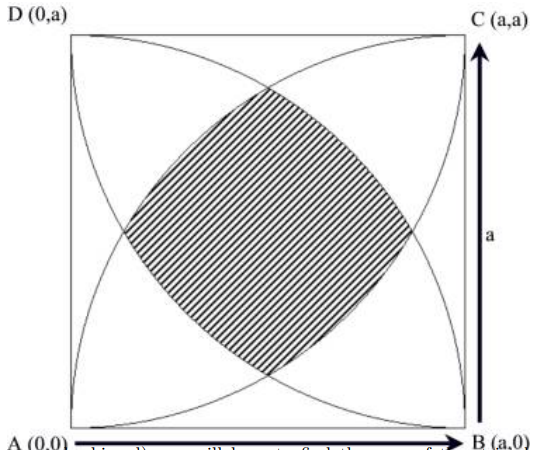
\includegraphics[width=1\textwidth]{img/area_uva}
    \column{.6\textwidth}
    {\bf QUIZ:}
    \begin{itemize}
      \item What is the area of the shaded part?
      \item You know $a$, the radius of the 4 circles;
    \end{itemize}\bigskip

    \begin{block}{Monte Carlo Approach}
      \begin{itemize}
      \item Sample $N$ random points;
      \item Calculate proportion $p$ of points in area;
      \item Shaded area is $\frac{a^2}{p}$\bigskip

      \item Mote Carlo approach is useful in several problems!
      \end{itemize}
    \end{block}
  \end{columns}
\end{frame}


% one dim measures: radius, diameter, circumference
% central angle, sector, arc
% chord: if you know the points, how to find the points if you know center and line
\begin{frame}
  \frametitle{Other circle properties}
    \begin{center}
      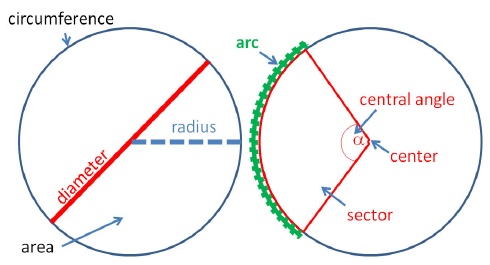
\includegraphics[width=0.6\textwidth]{../img/circle_halim0}
      \ppagenote{Circle Properties Images from Stephen Halim "Competitive Programming 3"}
    \end{center}

    \begin{itemize}
      \item {\bf radius:} $r$, {\bf diameter:} 2r, {\bf circumference:} $2\times\pi\times r$
      \item You can obtain $\pi$ from the problem, or with $\pi = 2\times \arccos(0)$
      \item Given a central angle $\alpha$:
      \begin{itemize}
        \item {\bf Arc:} $r\times\alpha$ (if in rad) or $r\times\frac{\alpha}{360}\times2\pi$ (if degrees)
        \item {\bf Sector:} $\frac{\alpha r^2}{2}$ (if in rad) or $2\pi r^2 \times \frac{\alpha}{360}$ (if degrees)
      \end{itemize}
    \end{itemize}
\end{frame}

\begin{frame}
  \frametitle{Other circle properties -- chord}
  \centering
    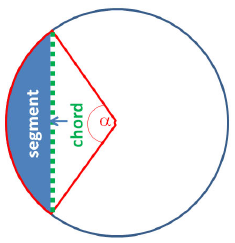
\includegraphics[width=0.3\textwidth]{../img/circle_halim1}

  \begin{itemize}
  \item {\bf chord:} Line segment with two ends in the circle's border.
  \item If you know $p_1$, $p_2$ and $c$, you can find $\alpha$ from the "angle" function;
  \item If you know $\alpha$ and $r$, you can find the size of the chord by: $|p_1p_2| = 2\times r\times\sin(\alpha/2)$
  \begin{itemize}
    \item {\bf Quiz:} If you know a line and a circle, how do you find $p_1$ and $p_2$?
  \end{itemize}
  \item If you know $p_1$, $p_2$, and $r$ (but not $\alpha$ or $c$), you can find the center of the circle using the code in the next page;
  \end{itemize}
\end{frame}

\begin{frame}[fragile]{Circle Center from points and radius}
  You have two points $p_1, p_2$ that form a chord in a circle, and the radius of that circle. How do you find the center?

  {\smaller
\begin{exampleblock}{}
\begin{verbatim}
bool circle2PtsRad(point p1, point p2, double r, point &c) {
  double d2 = (p1.x - p2.x) * (p1.x - p2.x) +
              (p1.y - p2.y) * (p1.y - p2.y);
  double det = r * r / d2 - 0.25;

  if (det < 0.0) return false; // Can't make circle

  double h = sqrt(det);
  c.x = (p1.x + p2.x) * 0.5 + (p1.y - p2.y) * h;
  c.y = (p1.y + p2.y) * 0.5 + (p2.x - p1.x) * h;
  return true;
}
// to get the other center, reverse p1 and p2
\end{verbatim}
\end{exampleblock}
  }
\end{frame}

\subsection{Triangles}

\begin{frame}
  \frametitle{Problem Example: 11909 - Soya milk}
  \begin{block}{How do you solve it?}
    \begin{itemize}
    \item {\bf Input}:\\
      The dimensions of a Milk box, and its inclination:\\
      $l, w, h, \theta$
    \item {\bf Output}:\\
      The amount of milk left in the box.
    \end{itemize}
  \end{block}

  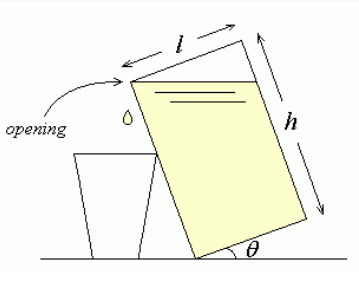
\includegraphics[width=0.4\textwidth]{img/milk_uva}
\end{frame}

\begin{frame}[t]
  \frametitle{Example: 10577 - Bounding Box}
  \begin{block}{}
    \begin{itemize}
      \item {\bf Input}: Three points that are the vertices of a {\bf regular polygon}, and number $n$ of sides in the polygon;\medskip
      \item {\bf Output}: Area of smallest {\bf axis aligned} rectangle that bounds this polygon.\medskip
      \item How do you solve it?
    \end{itemize}
  \end{block}
\end{frame}

\begin{frame}
  \frametitle{Triangle Basic Facts}

    \begin{itemize}
    \item {\bf Triangle Inequality}: If $a,b,c$ are sides of a triangle, then $a+b > c; a+c > b; b+c > a$;\bigskip
    \item {\bf Perimeter, Semiperimeter}: $p = a+b+c$, $s = p/2$\bigskip
    \item {\bf Area}: $A = \frac{bh_b}{2}$\bigskip
    \item {\bf Area (Heron's formula)}: $A = \sqrt{s(s-a)(s-b)(s-c)}$\bigskip
    \item {\bf Triangulation}: Any 2D polygon can be decomposed into triangles;
  \end{itemize}
\end{frame}

\subsection{incircle}
\begin{frame}[fragile]{Incircle of a Triangle}
    \begin{columns}
      \column{0.2\textwidth}
      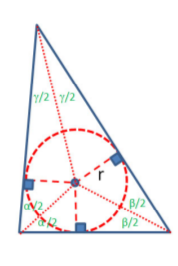
\includegraphics[width=1\textwidth]{../img/incircle_halim}
      \column{0.8\textwidth}
      \begin{itemize}
        \item An {\bf Inscribed Circle (incircle)} is the largest circle that fits inside a triangle;
        \item The radius of the incircle is: $r = A / s$
        \item The center of the circle can be found by the intersection of two {\bf angle bisectors}.
      \end{itemize}
      \end{columns}

    \begin{exampleblock}{Radius of the Incircle: $r = \text{area}/s$}
      {\smaller
\begin{verbatim}
double rInCircle(double ab, double bc, double ca) {
  return area(ab, bc, ca) / (0.5 * perimeter(ab, bc, ca)); }

double rInCircle(point a, point b, point c) {
  return rInCircle(dist(a, b), dist(b, c), dist(c, a)); }
\end{verbatim}}

    \end{exampleblock}
\end{frame}

\begin{frame}[fragile]
  \frametitle{Finding the center of the Incircle of a triangle}
  {\smaller
    \begin{exampleblock}{}
\begin{verbatim}
int inCircle(point p1, point p2, point p3,
             point &ctr, double &r) {
  r = rInCircle(p1, p2, p3);
  if (fabs(r) < EPS) return 0; // colinear points;
  line l1, l2; // compute these two angle bisectors

  double ratio = dist(p1, p2) / dist(p1, p3);
  point p = translate(p2, scale(toVec(p2, p3),
                      ratio / (1 + ratio)));
  pointsToLine(p1, p, l1);                // bisector 1

  ratio = dist(p2, p1) / dist(p2, p3);
  p = translate(p1, scale(toVec(p1, p3),
                ratio / (1 + ratio)));    // bisector 2
  pointsToLine(p2, p, l2);

  areIntersect(l1, l2, ctr);              // find center (ctr)
  return 1;
}
\end{verbatim}
    \end{exampleblock}
    }
\end{frame}

\begin{frame}
  \frametitle{Circumcircle of a Triangle}
  \begin{columns}
    \column{0.3\textwidth}
    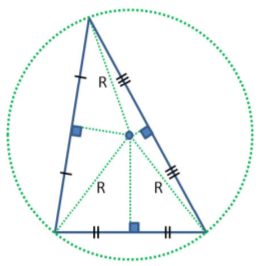
\includegraphics[width=1\textwidth]{../img/circumcircle_halim}
    \column{0.7\textwidth}
    \begin{itemize}
      \item The radius of the circumcircle in a triangle with sides $a,b,c$ and area A is $R = \frac{abc}{4A}$;
      \item The radius $R$ is also related to the {\bf Law of Sines}:
      \begin{equation*}
        \frac{a}{\sin{\alpha}} = \frac{b}{\sin{\beta}} = \frac{c}{\sin{\gamma}} = 2R
      \end{equation*}
    \end{itemize}
    \end{columns}\bigskip
    \begin{itemize}
      \item To find the center of the circumcircle:
      \begin{itemize}
        \item Use a similar algorithm as the center of the incirle (last slide);\medskip
        \item Instead of angle bisectors, use {\bf perpendicular bisectors};
      \end{itemize}
    \end{itemize}
\end{frame}

\section{Polygons}
\begin{frame}[fragile]
  \frametitle{Polygons -- Definition and data structure}

    A polygon is a plane figure bounded by a finite sequence of line
    segments.

  \begin{exampleblock}{Polygon Representation}
    \begin{itemize}
    \item In general, we store an array of points of the segments;
    \item We want to sort the points in CW or CCW order;
    \item Add the first point at the end of the array to avoid
      special cases;
    \end{itemize}
{\smaller
\begin{verbatim}
// 6 points, entered in counter clockwise order;
vector<point> P;
P.push_back(point(1, 1)); // P0
P.push_back(point(3, 3)); // P1
P.push_back(point(9, 1)); // P2
P.push_back(point(12, 4)); // P3
P.push_back(point(9, 7)); // P4
P.push_back(point(1, 7)); // P5
P.push_back(P[0]); // important: loop back
\end{verbatim}}
\end{exampleblock}
\end{frame}

\begin{frame}[fragile]
  \frametitle{Characteristics of a Polygon}
  {\smaller
    \begin{exampleblock}{Perimeter of a Poligon -- add the distances of the segments}
\begin{verbatim}
double perimeter(const vector<point> &P) {
  double result = 0.0;
  for (int i = 0; i < (int)P.size()-1; i++)
     // remember: P[0] = P[P.size()-1]
     result += dist(P[i], P[i+1]);
  return result; }
\end{verbatim}
    \end{exampleblock}

    \begin{exampleblock}{Area of a Poligon -- half of the determinant of the XY matrix of segments}
\begin{verbatim}
double area(const vector<point> &P) {
  double result = 0.0, x1, y1, x2, y2;
  for (int i = 0; i < (int)P.size()-1; i++) {
    x1 = P[i].x; x2 = P[i+1].x;
    y1 = P[i].y; y2 = P[i+1].y;
    result += (x1 * y2 - x2 * y1); }
  return fabs(result) / 2.0; }
\end{verbatim}
    \end{exampleblock}
}
\end{frame}


\begin{frame}[fragile]
  \frametitle{Testing if a Polygon is Convex}
  \begin{itemize}
    \item A convex polygon has no "holes";
    \item For any 2 points $p_1,p_2$ inside the polygon, segment is inside polygon too.
  \end{itemize}

    {\smaller
    \begin{exampleblock}{Easier Convex Testing: Every angle turns the same way}
\begin{verbatim}
bool isConvex(const vector<point> &P) {
  // Returns true if every 3 neighb vertices turn the same way;
  int sz = (int)P.size();
  if (sz <= 3) return false; // Not a polygon

  bool isLeft = ccw(P[0], P[1], P[2]); // described earlier

  for (int i = 1; i < sz-1; i++)
    if (ccw(P[i],P[i+1],P[(i+2) == sz ? 1 : i+2]) != isLeft)
      return false;            // not same direction as isLeft.

  return true;
}
\end{verbatim}
    \end{exampleblock}
  }
\end{frame}

\begin{frame}[fragile]
  \frametitle{Polygon -- Test point inside the polygon}
    % \begin{block}{There are many ways to test if a point $P$ is in a polygon.}
    %   \begin{itemize}
    %   \item \structure{Winding Algorithm}: Sum the angles of all
    %     angles $APB$ ($A,B$) are points in the polygon. If the sum is
    %     $2\pi$. Point is in polygon.
    %   \item \structure{Ray Casting Algorithm}: Draw an segment from
    %     $P$ to infinity, and count the number of polygon edges
    %     crossed. Odds: Inside. Even: Outside.
    %   \end{itemize}
    % \end{block}

  We can use the same idea to test if a point is inside the polygon: The direction of the point in relation to every edge should be the same.

    {\smaller
    \begin{exampleblock}{Winding Algorithm Code for point in polygon detection}
\begin{verbatim}
bool inPolygon(point pt, const vector<point> &P) {
  if ((int)P.size() == 0) return false;
  double sum = 0;

  for (int i = 0; i < (int)P.size()-1; i++) {
    if (ccw(pt, P[i], P[i+1]))
      sum += angle(P[i], pt, P[i+1]);       //left turn/ccw
      else sum -= angle(P[i], pt, P[i+1]);  //right turn/cw
  }

  return fabs(fabs(sum) - 2*PI) < EPS;
}
\end{verbatim}
    \end{exampleblock}
  }

  {\bf QUIZ:} What happens if the point is at an edge segment?
\end{frame}

\begin{frame}[fragile]
  \frametitle{Polygon -- Cutting}
  % TODO: Add an image explaining Polygon cutting
  {\smaller
    \begin{block}{}
      To cut $P$ along a line $AB$, we separate the points in $P$ to the
      left and right of the line.
    \end{block}

{\smaller
    \begin{exampleblock}{}
\begin{verbatim}
point lineIntersectSeg(point p, point q, point A, point B) {
  double a=B.y-A.y; double b=A.x-B.x; double c=B.x*A.y-A.x*B.y;
  double u=fabs(a*p.x+b*p.y+c); double v=fabs(a*q.x+b*q.y+c);
  return point((p.x*v + q.x*u)/(u+v),
               (p.y*v + q.y*u)/(u+v)); }

vector<point> cutPolygon(point a, point b, const vector<point> &Q){
  vector<point> P;
  for (int i = 0; i < (int)Q.size(); i++) {
    double left1 = cross(toVec(a, b), toVec(a, Q[i])), left2 = 0;
    if (i != (int)Q.size()-1)
      left2 = cross(toVec(a, b), toVec(a, Q[i+1]));
    if (left1 > -EPS)
      P.push_back(Q[i]); //Q[i] is on the left of ab
    if (left1*left2 < -EPS) //edge (Q[i], Q[i+1]) crosses line ab
      P.push_back(lineIntersectSeg(Q[i], Q[i+1], a, b)); }
  if (!P.empty() && !(P.back() == P.front()))
    P.push_back(P.front()); // make P's first point = P's last point
  return P; }
\end{verbatim}
    \end{exampleblock}}
  }
\end{frame}

\begin{frame}
  \frametitle{Polygon -- Convex Hull}

  \begin{itemize}
    \item A common problem: Given a set of points $S$, what is the {\bf smallest convex polygon} that includes all points in $S$?\bigskip

    \item One way to find the Convex Hull: for each point $p \in S$, determine if the point is at the edge of the polygon (in the hull) or inside the polygon (not in the hull).\bigskip

    \item We will introduce the $O(n\log n)$ algorithm "Graham's Scan"
  \end{itemize}

    \begin{center}
      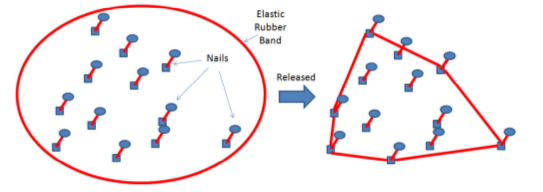
\includegraphics[width=.8\textwidth]{../img/convexhull_halim}
      \ppagenote{Convex Hull image by Steven Halim "Competitive Programming 3"}
    \end{center}
\end{frame}

\begin{frame}[fragile]
  \frametitle{Polygon -- Graham's Scan}
  \framesubtitle{Helper Functions -- sort two points based on their angle against the X axis}

{\small
\begin{exampleblock}{}
\begin{verbatim}
point pivot(0, 0);

bool angleCmp(point a, point b) {
  // special case: if collinear, choose closet to pivot;
  if (collinear(pivot, a, b)) // special case
    return dist(pivot, a) < dist(pivot, b);

  // calculate angle against the X axis:
  double d1x = a.x - pivot.x, d1y = a.y - pivot.y;
  double d2x = b.x - pivot.x, d2y = b.y - pivot.y;

  return (atan2(d1y, d1x) - atan2(d2y, d2x)) < 0;
}
\end{verbatim}
\end{exampleblock}
}
\end{frame}

\begin{frame}[fragile]
  \frametitle{Polygon -- Graham's Scan}
  \framesubtitle{Convex Hull -- Initializing the algorithm}

  {\small
    \begin{exampleblock}{}
\begin{verbatim}
vector<point> CH(vector<point> P) {
  int i, j, n = (int)P.size();
  // Special Case: Polygon with 3 points
  if (n <= 3) {
    if (!(P[0]==P[n-1])) P.push_back(P[0]);
    return P; }

  // Find Initial Point: Low Y then Right X
  int P0 = 0;
  for (i = 1; i < n; i++)
    if (P[i].y < P[P0].y ||
        (P[i].y == P[P0].y && P[i].x > P[P0].x))
      P0 = i;
  point temp = P[0]; P[0] = P[P0]; P[P0] = temp;
\end{verbatim}
\end{exampleblock}}
\end{frame}

\begin{frame}[fragile]
  \frametitle{Polygon -- Graham's Scan}
  \framesubtitle{Convex Hull -- More initialization}
  {\small
    \begin{exampleblock}{}

\begin{verbatim}

  // second, sort points by angle with pivot P0
  pivot = P[0];
  sort(++P.begin(), P.end(), angleCmp);

  // S holds the Convex Hull
  // We initialize it with first three points
  vector<point> S;
  S.push_back(P[n-1]);
  S.push_back(P[0]);
  S.push_back(P[1]);

  // We start on the third point
  i = 2;
\end{verbatim}

    \end{exampleblock}
  }
\end{frame}

\begin{frame}[fragile]
  \frametitle{Polygon -- Graham's Scan}
  \framesubtitle{Convex Hull -- Main Loop}

Now that we selected a pivot and sorted the points, we test every three points (following the sort) if they are in the convex hull.

  {\small
    \begin{exampleblock}{}
\begin{verbatim}
  while (i < n) {
    j = (int)S.size()-1;

    // If the next point is left of CH, keep it.
    // Else, pop the last CH point and try again.

    if (ccw(S[j-1], S[j], P[i]))
      S.push_back(P[i++]);
    else
      S.pop_back();
    }
  return S;
}                 // End Graham's Scan CH
\end{verbatim}
\end{exampleblock}}
\end{frame}
%% TODO: Add polygon problem example
